\documentclass[border=12pt]{standalone}
\usepackage{tikz}
\usepackage{amsmath,amssymb}
\usetikzlibrary{calc,decorations.pathreplacing,arrows.meta}
\begin{document}
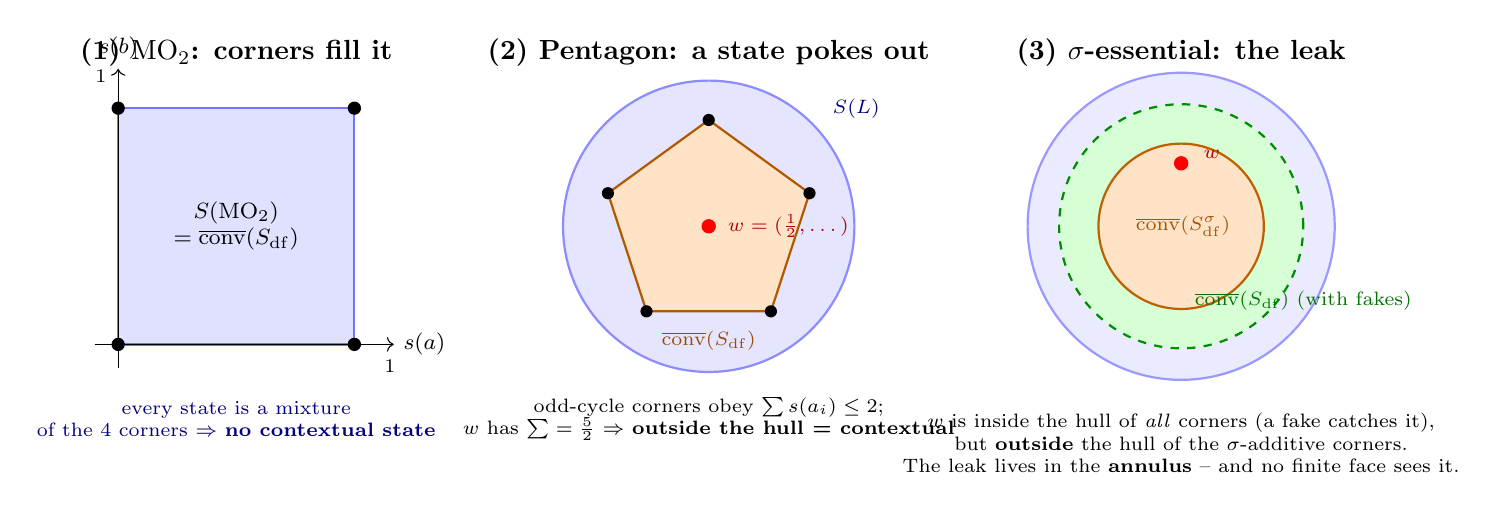
\begin{tikzpicture}[scale=1.0]

% ======================= PANEL 1: MO2 — corners fill the square =======
\begin{scope}[shift={(0,0)}]
  \node[anchor=south] at (1.5,3.4) {\textbf{(1) $\mathrm{MO}_2$: corners fill it}};
  % the square = state space [0,1]^2
  \fill[blue!12] (0,0) rectangle (3,3);
  \draw[blue!55,thick] (0,0) rectangle (3,3);
  \draw[->] (-0.3,0)--(3.5,0) node[right]{\footnotesize $s(a)$};
  \draw[->] (0,-0.3)--(0,3.5) node[above]{\footnotesize $s(b)$};
  % four dispersion-free corners
  \foreach \x/\y in {0/0,3/0,0/3,3/3}{\fill[black] (\x,\y) circle (2.4pt);}
  \node[font=\scriptsize] at (3.45,-0.28){$1$}; \node[font=\scriptsize] at (-0.22,3.4){$1$};
  \node[font=\footnotesize,align=center] at (1.5,1.5)
    {$S(\mathrm{MO}_2)$\\$=\overline{\mathrm{conv}}(S_{\mathrm{df}})$};
  \node[font=\scriptsize,align=center,blue!50!black] at (1.5,-0.95)
    {every state is a mixture\\of the 4 corners $\Rightarrow$ \textbf{no contextual state}};
\end{scope}

% ======================= PANEL 2: pentagon — hull pinched, state pokes out
\begin{scope}[shift={(6.0,0)}]
  \node[anchor=south] at (1.5,3.4) {\textbf{(2) Pentagon: a state pokes out}};
  % schematic: the fat state space (light), the pinched corner-hull (dark) inside it
  \fill[blue!10] (1.5,1.5) circle (1.85);                 % full state space S(L) (fat)
  \draw[blue!45,thick] (1.5,1.5) circle (1.85);
  % corner-hull = inner pentagon (the corners satisfy Sum<=2, pinched inward)
  \fill[orange!22]
    (1.5,2.85) -- (2.78,1.92) -- (2.29,0.42) -- (0.71,0.42) -- (0.22,1.92) -- cycle;
  \draw[orange!70!black,thick]
    (1.5,2.85) -- (2.78,1.92) -- (2.29,0.42) -- (0.71,0.42) -- (0.22,1.92) -- cycle;
  \foreach \p in {(1.5,2.85),(2.78,1.92),(2.29,0.42),(0.71,0.42),(0.22,1.92)}
    {\fill[black] \p circle (2.2pt);}
  % the contextual state: the 1/2-everywhere state, OUTSIDE the corner-hull
  \fill[red] (1.5,1.5) circle (2.6pt);
  \node[red!70!black,font=\scriptsize,anchor=west] at (1.62,1.5){$w=(\tfrac12,\dots)$};
  \node[orange!60!black,font=\scriptsize] at (1.5,0.05){$\overline{\mathrm{conv}}(S_{\mathrm{df}})$};
  \node[blue!50!black,font=\scriptsize,anchor=west] at (2.95,3.0){$S(L)$};
  \node[font=\scriptsize,align=center] at (1.5,-0.95)
    {odd-cycle corners obey $\sum s(a_i)\le2$;\\
     $w$ has $\sum=\tfrac52$ $\Rightarrow$ \textbf{outside the hull = contextual}};
\end{scope}

% ======================= PANEL 3: the sigma-essential annulus ==========
\begin{scope}[shift={(12.0,0)}]
  \node[anchor=south] at (1.5,3.4) {\textbf{(3) $\sigma$-essential: the leak}};
  \fill[blue!8] (1.5,1.5) circle (1.95);                  % all states
  \draw[blue!40,thick] (1.5,1.5) circle (1.95);
  % conv(S_df): ALL dispersion-free corners (incl. fakes) -- bigger hull (outer)
  \fill[green!16] (1.5,1.5) circle (1.55);
  \draw[green!55!black,thick,dashed] (1.5,1.5) circle (1.55);
  % conv(S_df^sigma): only sigma-additive corners -- smaller hull (inner)
  \fill[orange!22] (1.5,1.5) circle (1.05);
  \draw[orange!75!black,thick] (1.5,1.5) circle (1.05);
  % the witness state: in the annulus -- inside conv(S_df), outside conv(S_df^sigma)
  \fill[red] (1.5,2.30) circle (2.6pt);
  \node[red!70!black,font=\scriptsize,anchor=west] at (1.66,2.42){$w$};
  \node[orange!65!black,font=\scriptsize] at (1.5,1.5){\,$\overline{\mathrm{conv}}(S_{\mathrm{df}}^\sigma)$};
  \node[green!45!black,font=\scriptsize,anchor=west] at (1.55,0.55){$\overline{\mathrm{conv}}(S_{\mathrm{df}})$ (with fakes)};
  \node[font=\scriptsize,align=center] at (1.5,-1.25)
    {$w$ is inside the hull of \emph{all} corners (a fake catches it),\\
     but \textbf{outside} the hull of the $\sigma$-additive corners.\\
     The leak lives in the \textbf{annulus} -- and no finite face sees it.};
\end{scope}

\end{tikzpicture}
\end{document}
